\documentclass[a4paper,11pt]{article}

\usepackage{graphicx}          
\usepackage{amsmath}         

\usepackage[top=30mm, bottom=30mm, left=20mm, right=20mm, columnsep=20pt]{geometry} % Document margins
\usepackage[colorlinks,bookmarks=false]{hyperref}

\usepackage[utf8]{inputenc}  
\usepackage[english]{babel}    
\usepackage{subfigure}
\usepackage[justification=centering]{caption}
\usepackage{abstract}
\usepackage{amssymb}
\usepackage{listings}
\usepackage{epstopdf}

\usepackage[backend=bibtex,sorting=none,firstinits=true,isbn=false,doi=false]{biblatex}
\addbibresource{report.bib}

%===============================================================================
%===============================================================================
\begin{document}

\begin{titlepage}
\date{}
\begin{figure}
\centering

\includegraphics[scale=0.35]{figures/KTH_Logo.png}
\end{figure}
\title{
\vspace{-1cm}
\textsc{DD2425 - Robotics and Autonomous Systems}
\\
\vspace{0.5cm}
\textsc{Group 6}\\
{\large \today}
\begin{center}
\rule{\linewidth}{0.5mm}
\textbf{Project Report}
\rule{\linewidth}{0.5mm}
\end{center}
}
\maketitle
\vspace{-2cm}
\begin{figure}[h]
\centering
\begin{minipage}[b]{0.3\linewidth}
                \begin{flushleft}
\normalsize{
\emph{Authors}\\
\vspace{0.5cm}
Carlos \textsc{Gálvez del Postigo} \\
Mathias \textsc{Lindblom} \\
Tingyu \textsc{Liu} \\
Gundars \textsc{Kalns}
}
\end{flushleft}
\end{minipage}
\qquad
\quad
\begin{minipage}[b]{0.62\linewidth}
                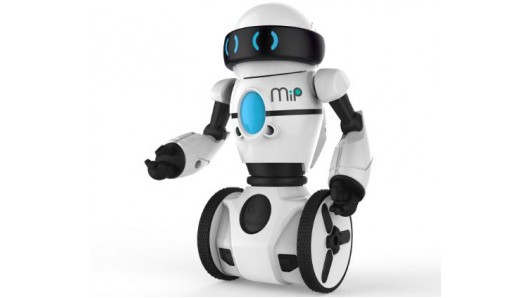
\includegraphics[width=\linewidth]{figures/robot.jpg}
\end{minipage}
\end{figure}
\vspace{1cm}
\thispagestyle{empty}
\begin{abstract}
This report describes the work done for the Robotics and Autonomous Systems project. The task consisted on designing a robot that would be able to autonomously explore a maze, avoid obstacles, detected and identify objects and build a map as it navigates. In addition, on a second run, it had to be able to "fetch" the objects as fast as possible using the previously acquired knowledge. The robot was tested in the laboratory and in a contest with satisfactory results. Finally, a performance analysis and some conclusions summarize this report. 
\end{abstract}
\end{titlepage}

%===============================================================================
\begingroup
\hypersetup{linkcolor=black}
\tableofcontents
\endgroup
\newpage

%===============================================================================
\section{Introduction\label{sec:Introduction}}
This report describes the work done for the final project for the course Robotics and Autonomous systems. The purpose is to reflect about ideas and solutions we provided in order to try to reach the goal of this course – making autonomous robot that can explore maze, create map of it and detect and recognize different geometrical objects located in maze.


%===============================================================================
\section{Mechanical design \label{sec:Mechanics}}
The robot was built following a standard differential drive configuration (XXXX reference) because of an easier control (e.g.: rotate around it's center point without moving). A picture of the robot can be seen in Figure \ref{fig:robotPic}.

\begin{figure}[h]
        \centering
        \begin{subfigure}[b]{0.45\linewidth}
        \centering
                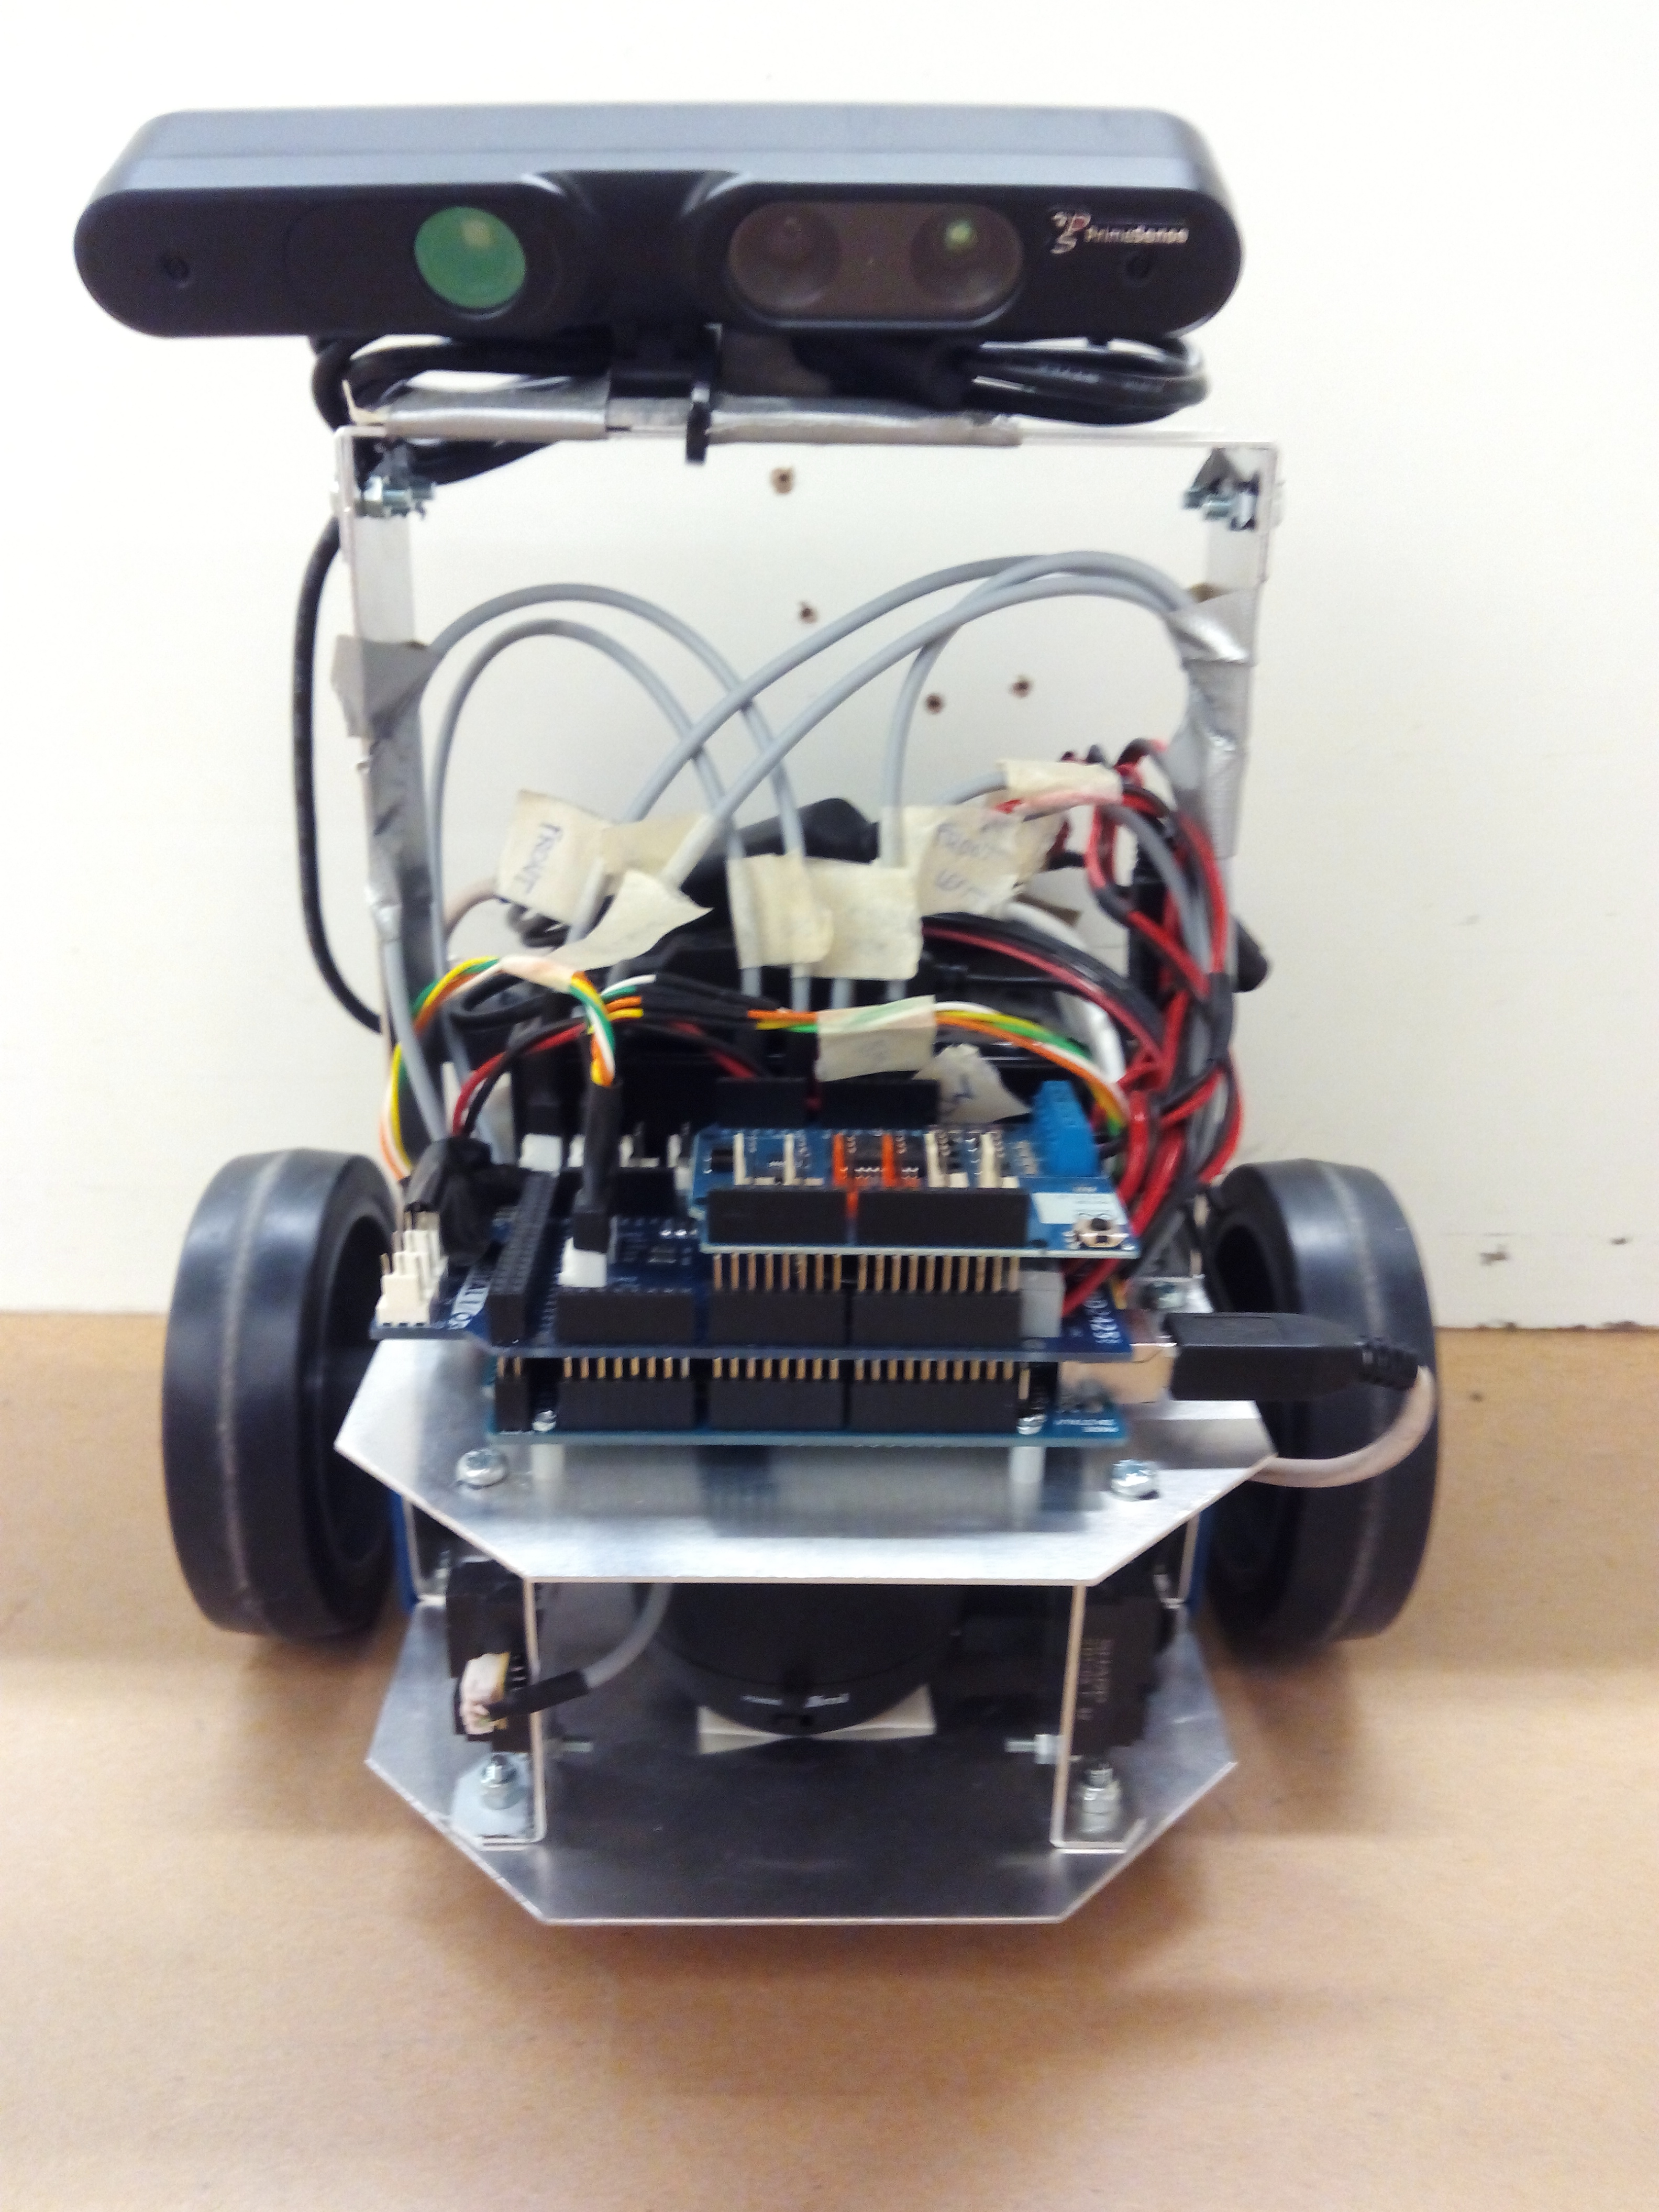
\includegraphics[height=5cm]{figures/front.jpg}
		\caption{Front view}
        \end{subfigure}
        \begin{subfigure}[b]{0.45\linewidth}
        \centering
                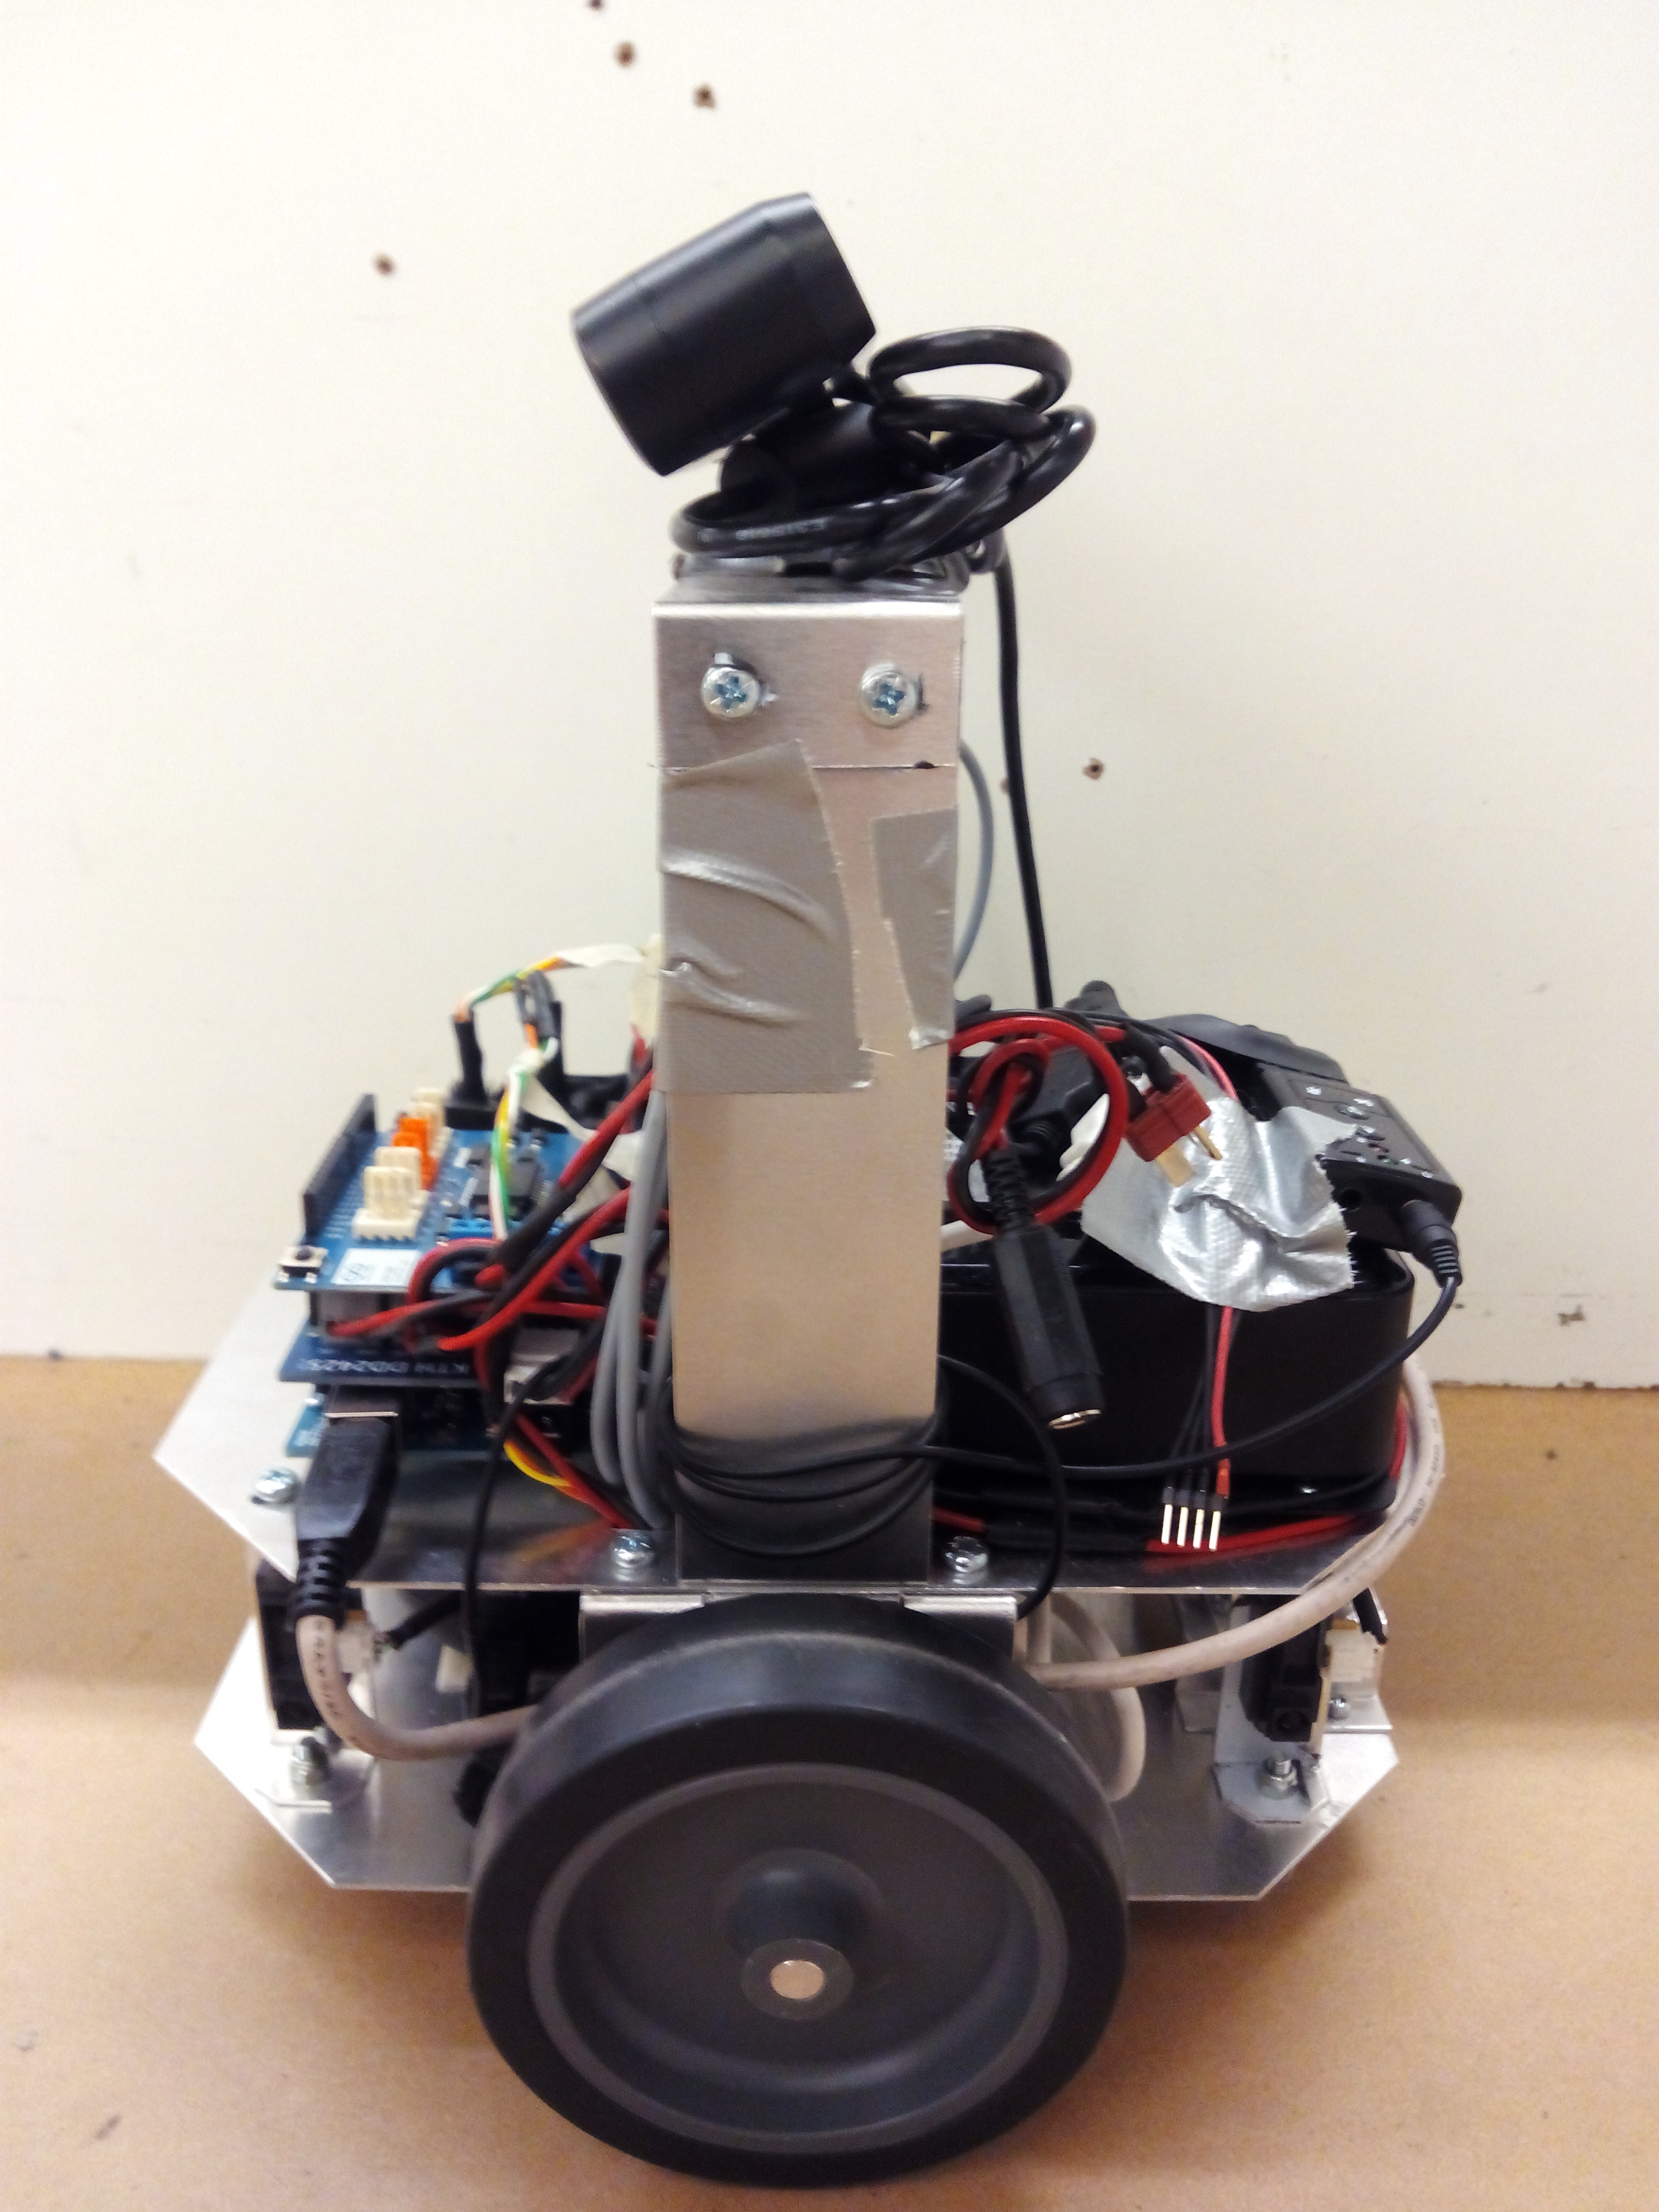
\includegraphics[height=5cm]{figures/side.jpg}
                \caption{Side view}
        \end{subfigure}
        \caption{Pictures of the robot}
                \label{fig:robotPic}
\end{figure}


The dimensions are 23 cm x 23 cm wide and long (including wheels) and 29 cm high. Two aluminium plates are connected with four pillars in order to create two floors. On the first floor are located motors, the battery and speaker whereas on the second floor the NUC and the Arduino sandwich can be found. For camera there is pillar which raises it high enough so it reaches 29 cm height. This is required in order to get depth information, which requires a minimum distance of 35 cm from the camera. The IMU is located at the center of the robot, under the second plate, as well as the long range IR sensors looking forward and backwards. The short range IR sensors are located on the pillars which connect first and second floor, with the aim of performing wall following. 

%===============================================================================


%===============================================================================


%===============================================================================
\newpage
\printbibliography 

\end{document}